\section*{Redes Neuronais Artificiais}\label{sec:RNA}

Nos dias de hoje abundam as plataformas e ferramentas disponíveis no mercado para o estudo e desenvolvimento de Redes Neuronais Artificiais. Desde aplicações específicas, bibliotecas para linguagens, até linguagens criadas especificamente para trabalhar e lidar com Inteligência Artificial. Torna-se, por isso cada vez mais uma questão de que linguagem de programação usar, qual é que vai cumprir melhor a sua tarefa.
\\
Além disso, e embora nos situemos num contexto académico torna-se importante pensar mais além e ter a noção da diferença entre as plataformas usadas para investigação e aprendizagem daquelas que terão que cumprir um papel real em situações reais, quando implementadas em contextos de produção. São de seguida exploradas três linguagens: \textit{R}, \textit{Python} e \textit{Julia}, apresentando para cada uma dessas um estudo sobre uma biblioteca de manipulação de RNAs.


\subsection*{Linguagem R}

\textit{R} é uma linguagem e um ambiente de desenvolvimento integrado muito usado para cálculos estatísticos e gráficos. Torna-se por isso menos flexível e compatível comparando com outras, como por exemplo o \textit{Python}. É uma linguagem bastante especializada no campo da estatística e menos prática para ser usada em contextos mais abrangentes do que uma investigação académica.\\
Contudo, uma das grandes vantagens da linguagem \textit{R} são os tipos nativos e a facilidade de representação de tipos complexos como por exemplo vetores e matrizes, não havendo a necessidade de recursos adicionais para a sua representação.\\
Outro dos pontos fortes da linguagem é a quantidade de bibliotecas disponíveis para uso, apresentando uma vasta escolha no que toca a Redes Neuronais. Além disso, a facilidade de criação e manipulação de gráficos nativamente é outro dos pontos fortes. Por sua vez, limitações nas opções de personalização do hardware a usar são pontos negativos do \textit{R}, por exemplo, não é possível escolher nativamente entre o CPU e GPU para o treino das redes.
Uma das bibliotecas mais usadas no que toca a RNA é a \textit{NeuralNet}, usada para treino das redes e que apresenta bastante personalização e reutilização.

\vspace{5mm}

\begin{lstlisting}[breaklines,caption=NeuralNet,frame=tlrb,language=r]{Name}
neuralnet(formula, data, hidden = 1, threshold = 0.01,
    stepmax = 1e+05, rep = 1, startweights = NULL,
    learningrate.limit = NULL,
    learningrate.factor = list(minus = 0.5, plus = 1.2),
    learningrate=NULL, lifesign = "none",
    lifesign.step = 1000, algorithm = "rprop+",
    err.fct = "sse", act.fct = "logistic",
    linear.output = TRUE, exclude = NULL,
    constant.weights = NULL, likelihood = FALSE)
\end{lstlisting}

\newpage

Alguns parâmetros de personalização do treino de uma Rede Neuronal na \textit{NeuralNet} são:

\begin{itemize}
    \item formula - a descrição do modelo a ser treinado
    \item data - os dados para treino da RNA
    \item hidden - o número de neurónios presentes em cada camada da rede
    \item threshold - valor numérico que especifica o limite para as derivadas parciais da função de erro e que funcionam como critério de paragem
    \item rep - número de repetições do treino da rede
    \item stepmax - número máximo de iterações para o treino da rede
    \item startweights - vetor que contém os valores inicias para os pesos dentro da rede, não sendo por isso inicializados aleatoriamente.
    \item learningrate.limit - vector ou lista contendo os máximos e mínimos para a taxa de aprendizagem. Usado para algoritmos RPROP e GRPROP.
    \item learningrate.factor - vector ou lista contendo os multiplicadores para os máximos e mínimos da taxa de aprendizagem nos algoritmos RPROP e GRPROP.
    \item learningrate - valor numérico que especifica a taxa de aprendizagem.
\end{itemize}

Para além disto é possível personalizar o algoritmo/método de aprendizagem que queremos usar na rede. A biblioteca \textit{NeuralNet} tem disponíveis vários algoritmos, entre eles:

\begin{itemize}
    \item Backpropagation
    \item Resilient Backpropagation
    \item Weight Backtracking 
    \item Modified Globally Convergent (GRPROP)
\end{itemize}

O resultado da execução do treino da rede neural é um objeto da classe nn e de onde podemos extrair a função de erro, a função de ativação, a lista de resultados por cada repetição do treino da rede e o modelo do treino.

\begin{figure}[H]
    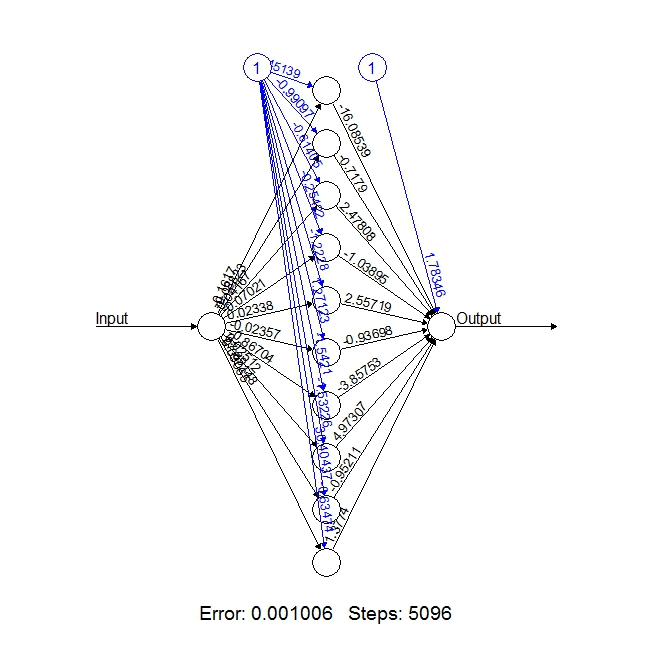
\includegraphics[scale=0.6]{tex/img/SquareRootNeuralNetImage.jpeg}
\end{figure}

\vspace{2mm} A \textit{NeuralNet} é apenas uma biblioteca disponível para o treino de Redes Neuronais Artificiais em R, existem outras como o \textit{MXNet}, \textit{nnet}, \textit{RSNNS} e \textit{H2O}.

\newpage

\subsection*{Python}

\textit{Python} é uma linguagem de programação multi-paradigma, que apresenta várias funcionalidades, flexibilidade, tornando-a muito apropriada para prototipar e testar hipóteses rapidamente. Por esta razão, \textit{Python} é cada vez mais escolhida no campo da Inteligência Artificial. Tal como explorado no \textit{R}, as bibliotecas disponíveis no Python são variadas e bastante úteis neste contexto.
\\Uma das bibliotecas mais usadas em \textit{Python} para a criação de Redes Neuronais Artificiais é o \textit{TensorFlow}, originalmente criada pela Google e open-source. A grande vantagem em relação a por exemplo, a \textit{NeuralNet} é o facto de ser muito mais versátil, aplicando-se a uma variedade de domínios muito maior. Para além disso, é possível executar em CPU, em GPU ou até mesmo em TPUs, uma unidade de processamento criada especificamente para o treino de Redes Neuronais com o \textit{Tensorflow}.

\begin{lstlisting}[breaklines,caption=TensorFlow,frame=tlrb,language=python]{Name}
# Parameters
learning_rate = 0.1
num_steps = 500
batch_size = 128
display_step = 100

# Network Parameters
n_hidden_1 = 256 # 1st layer number of neurons
n_hidden_2 = 256 # 2nd layer number of neurons
num_input = 784 # MNIST data input (img shape: 28*28)
num_classes = 10 # MNIST total classes (0-9 digits)

# tf Graph input
X = tf.placeholder("float", [None, num_input])
Y = tf.placeholder("float", [None, num_classes])

# Store layers weight & bias
weights = {
    'h1': tf.Variable(tf.random_normal([num_input, n_hidden_1])),
    'h2': tf.Variable(tf.random_normal([n_hidden_1, n_hidden_2])),
    'out': tf.Variable(tf.random_normal([n_hidden_2, num_classes]))
}
biases = {
    'b1': tf.Variable(tf.random_normal([n_hidden_1])),
    'b2': tf.Variable(tf.random_normal([n_hidden_2])),
    'out': tf.Variable(tf.random_normal([num_classes]))
}


# Create model
def neural_net(x):
    # Hidden fully connected layer with 256 neurons
    layer_1 = tf.add(tf.matmul(x, weights['h1']), biases['b1'])
    # Hidden fully connected layer with 256 neurons
    layer_2 = tf.add(tf.matmul(layer_1, weights['h2']), biases['b2'])
    # Output fully connected layer with a neuron for each class
    out_layer = tf.matmul(layer_2, weights['out']) + biases['out']
    return out_layer

# Construct model
logits = neural_net(X)
prediction = tf.nn.softmax(logits)

# Define loss and optimizer
loss_op = tf.reduce_mean(tf.nn.softmax_cross_entropy_with_logits(
    logits=logits, labels=Y))
optimizer = tf.train.AdamOptimizer(learning_rate=learning_rate)
\end{lstlisting}

Como podemos observar pelo código acima, as opções de personalização do \textit{TensorFlow} são muito variadas. Podemos definir os parâmetros da rede: taxa de aprendizagem, número de passos, entre outros, podemos ainda definir a arquitetura da nossa rede, indicando o número de camadas e o número de neurónios por camada. e ainda selecionar o algoritmo com o qual queremos treinar a nossa rede, estão disponíveis vários algoritmos:

\begin{itemize}
    \item Optimizer
    \item GradientDescentOptimizer
    \item AdadeltaOptimizer
    \item AdagradOptimizer
    \item AdagradDAOptimizer
    \item MomentumOptimizer
    \item AdamOptimizer
    \item FtrlOptimizer
    \item ProximalGradientDescentOptimizer
    \item ProximalAdagradOptimizer
    \item RMSPropOptimizer
\end{itemize}

O \textit{Tensorflow} torna-se assim uma solução muito completa para a criação e treino de Redes Neuronais tanto em contextos científicos como em contextos de mercado, contudo e devido ao seu elevado grau de personalização poderá ter uma grande curva de aprendizagem inicial.

\begin{figure}[H]
    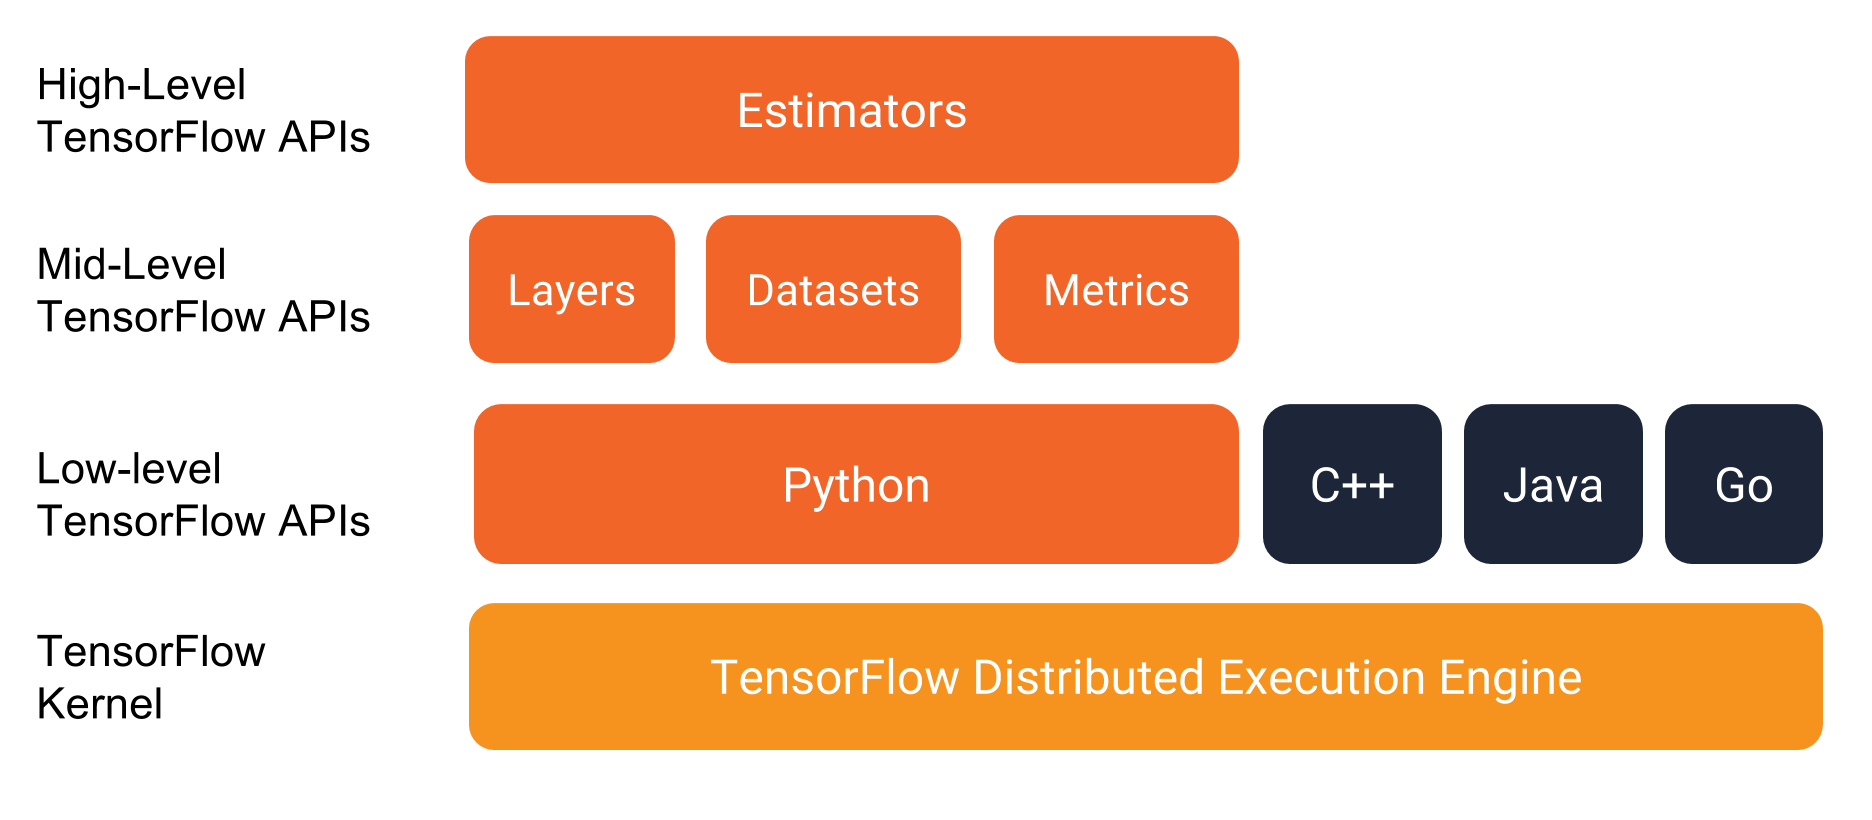
\includegraphics[scale=0.18]{tex/img/tensorflow_programming_environment.png}
\end{figure}

\vspace{2mm} O \textit{TensorFlow} é apenas uma biblioteca disponível para o treino de Redes Neuronais Artificiais em \textit{Python}, existem outras como \textit{Blocks}, \textit{Lasagne}, \textit{Keras}, \textit{Deepy}, \textit{Nolearn} e \textit{NeuPy}.

\subsection*{JULIA}

A linguagem \textit{Julia} foi criada com o foco em computação numérica, apresentando mesmo a possibilidade de fazer nativamente computação paralela distribuída. É por isso uma boa linguagem de programação para aplicações em que seja necessário muita computação, por exemplo para o treino de redes neuronais com grande quantidade de dados. Por outro lado, o facto de ser uma linguagem recente torna-a instável e não apresenta o mesmo número de bibliotecas disponíveis que o \textit{Python} ou o \textit{R}.
\\A principal biblioteca de Redes Neuronais Artificiais em \textit{Julia} é o \textit{MXNet}. Esta biblioteca permite o treino de Redes Neuronais distribuído por vários CPUs e GPUs.

\begin{lstlisting}[breaklines,caption=MXNet,frame=tlrb,language=python]{Name}
using MXNet

mlp = @mx.chain mx.Variable(:data)             =>
  mx.FullyConnected(name=:fc1, num_hidden=128) =>
  mx.Activation(name=:relu1, act_type=:relu)   =>
  mx.FullyConnected(name=:fc2, num_hidden=64)  =>
  mx.Activation(name=:relu2, act_type=:relu)   =>
  mx.FullyConnected(name=:fc3, num_hidden=10)  =>
  mx.SoftmaxOutput(name=:softmax)

# data provider
batch_size = 100
include(Pkg.dir("MXNet", "examples", "mnist", "mnist-data.jl"))
train_provider, eval_provider = get_mnist_providers(batch_size)

# setup model
model = mx.FeedForward(mlp, context=mx.cpu())

# optimization algorithm
optimizer = mx.SGD(learning_rate=0.1, momentum=0.9)

# fit parameters
mx.fit(model, optimizer, train_provider, n_epoch=20, eval_data=eval_provider)
\end{lstlisting}

As opções de personalização do \textit{MXNet} são bastantes. É possível definir a tipologia da rede, o objetivo de cada camada e os neurónios presentes. À semelhança do \textit{TensorFlow} em \textit{Python}, é possível aplicar vários modelos à Rede Neuronal em \textit{Julia}. Os modelos disponíveis são:

\begin{itemize}
    \item AbstractModel
    \item FeedForward
    \item Predict
    \item Fit
\end{itemize}

Além disso, é possível também escolher vários algoritmos de otimização:
\begin{itemize}
    \item AbstractOptimizer
    \item ADAM
    \item AdaGrad
    \item AdaDelta
    \item AdaMax
    \item RMSProp
    \item Nadam
\end{itemize}

O \textit{MXNet} tem mais duas grandes vantagens, para além de ser compatível com várias linguagens é também suportado por vários serviços de computação na nuvem como por exemplo AWS ou o Google Cloud.

\vspace{2mm} O \textit{MXNet} é apenas uma biblioteca disponível para o treino de Redes Neuronais Artificiais em \textit{Julia}, existem outras como o \textit{Mocha.jl}, o \textit{Tensorflow} e o \textit{KNet.jl}.

\subsection*{Outros}

\textit{R}, \textit{Python} e \textit{Julia} são apenas três linguagens onde se podem construir e treinar Redes Neuronais Artificiais, existem outras como por exemplo Matlab com a biblioteca NNet, C++ com a biblioteca OpenNN, Octave com a biblioteca Octave-NN e Java com a biblioteca NeuroPH.